\section{System overview}
\label{sec:design}

\Sys is view-centric, networking policies are nothing but derived
(virtual) DB views -- application-specific data selected and
restructured from the source (base) forwarding plane data, defined and
manipulated through DB operations.

% This section outlines the two enabling components: \TI that
% interfaces users with customer abstractions and \TR that processes
% operations.

% \Subsection{Data\hyp{}independent networking}
% \subsection{Network abstractions on demand}
% \subsection{Services}

\TI offers a two-level data abstraction, internal base tables for
network FIBs, and separate external views for simplifying user
operation.  \TI is centered around the external views, which offers
application-specific network-wide data-structures that are
customizability, virtual, and updatable.

\Paragraph{Views are customizable.} While base (stored) tables are
unified distributed over the network to achieve reasonable
performance, as we will discuss more in \TR. Views are the external
interface exposed to users, who can dynamically create and change
views by SQL queries that select relevant information from base
tables. Views also restructure the selected data to to simplify
operations.  
A particularly useful class of views are policy views: the view schema
structures the ``network-wide data'', specifying attributes of the
derived data item. \Eg the schema of \texttt{end\_to\_end policy} view
(Details in Table \ref{tb:endpoint}) is \nd{\{flow, ingress,
  egress\}}, structuring the view into three attributes. A view record
represents a policy instance, \eg \nd{(1,1,4)} directs that flow
\nd{1} entering the network by \nd{1} is to exit the network via
\nd{4}. Unlike the network-view in network-OS or programming APIs, in
\Sys, users have complete control over views, can create or destroy
views as needed, to simplify different applications at their will.

\Paragraph{Views are virtual.}  Views are derived from the base
tables, where the ``derivation relation'' is the SQL query that
generates the view. \Eg a specific routing decision in the
\nd{end\_to\_end policy} view is derived from the forwarding rules
stored in the base tables by a recursive query that computes
end-to-end reachability. Since the output of a SQL query is a table by
itself, views are used as the base tables, though only the view
definition is stored.  From performance perspective, a view consumes
zero resource until it is referred \ie queried by other programs. When
a view is queried, the stored SQL query is simply re-computed. This
treatment also keeps the view contents fresh, always reflecting the
latest network configuration. This process is called view
maintenance. Decades of DB query optimization have made view
maintenance very fast, enabling real-time network verification by
simply querying the views.

\Paragraph{Views are updatable} to enable network management directly
through views. For example, an administrator re-selecting a path for
all flows entering node \nd{1} to exit via \nd{3}
(Figure~\ref{fig:eg-one-big-switch}), only need to ``update'' the
\nd{end\_to\_end policy view} (\S~\ref{sec:details}) records, like the
following:
\begin{sql}
UPDATE e2e_policy SET egress = 3 WHERE ingress = 1;
\end{sql}
\Sys view update facility populates this update into the per\_switch \nd{configuration} base table, like the following:
\begin{sql}
UPDATE configuration SET next = 2 WHERE switch = 1;
UPDATE configuration SET next = 3 WHERE switch = 2;
\end{sql}
In general, view update which populates arbitrary modification to
views into to the base is a harder one: since views are derived from
the base, and in principle contains only partial information of the
base, a unique base table update that implements the view update does
not always exist. As a result, commercial DBS only supports updates
for a limited class of views when an unambiguous one-one mapping
between base and view exists.  In \Sys, however, we implement view
update for a larger family of views (\eg reachability) via triggers
(DBS's equivalent for call-back functions). We will revisit view
update in \S~\ref{sec:details}.


% \todo{(this subsection) HotNet texts, will rework}

% We first present \Sys's data abstractions. 
The data considered in \Sys is the forwarding plane consisting of all
the switch configurations, \ie FIB.  These ``distributed'' rules
naturally form \Sys \textit{base (stored) tables} and become \Sys's
internal representation of the network forwarding plane. Just like a
distributed network FIB is primarily designed for traffic processing,
the base tables are designed for transaction processing and are not exposed
to \Sys's end users. Externally, \Sys exposes a separate programmable
abstraction called \textit{(network)
  views}.  % Views are customizable,
% users are not confined to any pre-defined sets, user can create and
% destroy views on the fly. 
The customizable view is simply a SQL query which takes base tables as
input, and outputs a new virtual table. A view typically
contains network-wide data, \eg network data selected from nodes
belonging a path or a spanning tree, whichever relevant to a
particular user's task. The view data is also re-structured to simplify
user logic. In the following, we use an example network
(Figure~\ref{fig:eg-one-big-switch}) to illustrate the details.

% to optimize system performance, traffic processing, \eg throughput,
% not for the purpose of managing them from a user (administrator or a
% network application) perspective.
% To extract the data abstraction
% that best suits a user's demand on the fly, \Sys is designed to\\
% utilize DB view mechanism that allows a user to create abstraction on
% demand.  Specifically, the dataplane is treated as base (\ie stored)
% tables, whereas application data become user views derived from the
% base.
\vspace{-.5em}
\begin{figure}[ht!]
  \centering
  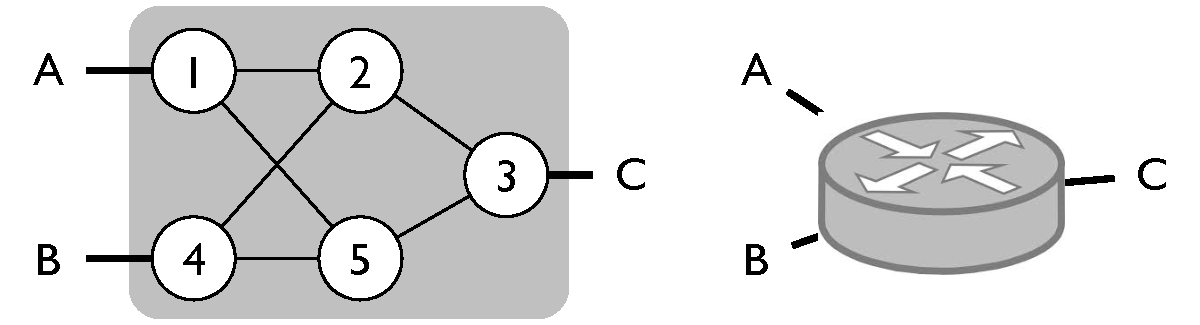
\includegraphics[width=.95\linewidth]{eg-one-big-switch.pdf}
  \caption{\footnotesize Example network and its one big switch
    abstraction}
  \label{fig:eg-one-big-switch}
\end{figure}
\vspace{-1em}

\Paragraph{As base tables} represent a network's
forwarding state, its role is to hide hardware heterogeneity, enable
transaction processing, and ease the creation of external
abstractions. Hence, they hold all the network
(configuration) data in a unified form that is easily accessible.  A
natural choice is a relational model~\cite{hull_relative_1984} that 
consists of three tables: \nd{topology} table that models network as a
pool of resource capacity, \nd{configuration} table that is the union
of all FIBs, and an optional \nd{constraint} table for 
network constraints (\eg SLAs).  \Eg Table~\ref{table:base-table}
shows example table instances.
% annotated topology table~\ref{tb:topology} represents the network's
% resource limit, whereas the flow table
% configuration~\ref{tb:configuration} is a snapshot of the network's
% allocated resource.
All tables are populated when the network is set up (assuming the FIBs
configured pro-actively), and incrementally updated afterwards as
network topology and/or configuration changes.

\begin{table}[ht!]
\begin{subtable}[t]{0.5\linewidth}
  {
    \footnotesize
    \subcaption{topology}
      \begin{tabular}[t!]{c|c|c|c}
        \centering
        node & node & avail\_bw  & used\_bw \\
        \hline
        1 & 2 & 3 & 2 \\
        1 & 5 & 5 & 0 \\
        \multicolumn{4}{c}{...}\\
        \hline
        4 & 5 & 5 & 0 \\
        4 & 2 & 5 & 0 \\ 
        \multicolumn{4}{c}{...}
        \label{tb:topology}
    \end{tabular}
  }
\end{subtable}
\;
\begin{subtable}[t]{0.45\linewidth}
  {
    \footnotesize
    \subcaption{per\_switch configuration}
    \centering
    \begin{tabular}[t]{c|c |c|c}
      \centering
      switch & flow & next & bw \\
      \hline
      1 & 1 & 2 & 1 \\
      1 & 2 & 2 & 1  \\
      \multicolumn{4}{c}{...}\\
      \hline
      2 & 1 & 3 & 1 \\
      \multicolumn{4}{c}{...}\\
      \hline
      3 & 1 & C & 1 \\
      \multicolumn{4}{c}{...}
      \label{tb:configuration}
    \end{tabular}
  }
\end{subtable}
\caption{\footnotesize Example base tables}
\label{table:base-table}
\end{table}
\vspace{-1em}

\Paragraph{The user-defined virtual views} are external
abstractions interfacing with users that are derived from the base tables as SQL
queries and serve as a logical perspective for a user's task. Compared to the
logical contexts introduced in earlier
works~\cite{ethane-sigcomm07,virtual-forwarding-plane}, the strength
of \Sys views is that it does not confine users to preselected
frozen abstractions, instead \Sys views can be created and changed by
users on demand by simply issuing or modifying a SQL query,
which selects from the distributed base tables the relevant
information and restructures them into a network-wide data-structure
that fits the user's task.

\begin{table}[ht!]
  \centering
\begin{subtable}[t]{0.3\linewidth}
    \centering
  {\footnotesize
    \subcaption{routing policy}
      \begin{tabular}[t]{c|c}
        flow & path\_vector \\
        \hline
        1 & (1,2,3) \\
        2 & (1,2,4) \\
        3 & (4,5,3) \\
        \multicolumn{2}{c}{...}
        \label{tb:routing} 
    \end{tabular}
    }
  \end{subtable}
  \;
  \begin{subtable}[t]{0.33\linewidth}
    \centering
  {\footnotesize
    \subcaption{end\_to\_end policy}
    \begin{tabular}[t]{c|c|c}
      flow & ingress & egress \\
      \hline
      1 & 1 & 3 \\
      2 & 1 & 4 \\
      3 & 4 & 3 \\
      \multicolumn{3}{c}{...}
      \label{tb:endpoint}
    \end{tabular}
    }
  \end{subtable}
  \;
  \begin{subtable}[t]{0.3\linewidth}
    \centering
  {\footnotesize
    \subcaption{one\_big\_switch}
    \begin{tabular}[t]{c|c}
        flow & next \\
        \hline
        1 &  C  \\
        2 & B \\
        3 & C \\
        \multicolumn{2}{c}{...}
        \label{tb:rule-capacity}
      \end{tabular}
    }
  \end{subtable}        
  \caption{\footnotesize Example views.}
\label{table:eg-views}
\end{table}

For example, a network-wide routing policy is nothing but the abstract
data as a view (Table~\ref{tb:routing}), derived from the per-switch
\nd{configuration} table, by the following query:
\begin{sql}
CREATE VIEW routing_policy AS (
  SELECT DISTINCT c.flow_id, fp.path_vector
  FROM configuration c 
       NATURAL JOIN flow_policy_fun(c.flow_id) fp
  ORDER BY c.flow_id );  
\end{sql}
In line 2, the \nd{select} statement selects two attributes to from
the view schema: attribute \nd{flow\_id} from \nd{configuration} and
\nd{path\_vector} from \nd{flow\_policy\_fun} which is a recursive
function that computes routing path for \nd{flow\_id}. 
% The \nd{JOIN} statement allows flows to be returned in the absence
% of configuration.  The resulting table of two attributes
% \nd{flow\_id} and \nd{path\_vector} forms the \nd{routing\_policy}
% view.
Similarly, we can derive a one-big-switch configuration view from
\nd{configuration} table and the \nd{obs\_mapping} table which keeps
tracks of the constituting physical nodes \nd{p\_node}.
\begin{sql}
CREATE VIEW obs_configuration AS (
  SELECT flow_id, t.next_id
  FROM   configuration t INNER JOIN obs_mapping ob
  ON     t.switch_id = ob.p_node );  
\end{sql}

Since a view is virtual, only its definition (the query) is stored.
Codd's relational model ensures that a SQL query outputs nothing but tables
(relations), allowing users to use views exactly as a table. A direct
usage is to create views on top of views. The next example shows how to
create an end-to-end policy (Table~\ref{tb:endpoint}) view from
\nd{routing\_policy} view:
\begin{sql}
CREATE VIEW e2e_policy AS (
 SELECT flow_id,
       path_vector[1] AS ingress,
       path_vector[array_length(path_vector,1)] AS egress
 FROM  routing_policy
 ORDER BY flow_id ) ;  
\end{sql}
